\documentclass[a4paper,twoside, openany,11pt]{book}
\usepackage{import}
\import{C:/Users/adrie/OneDrive/Programmation/LATEX/0_macro/Macro_2018_01_06/}{ensae_memoire.tex}

\programmationCPP

\newcommand{\PDGtitre}{Projet de C++ 2A}
\newcommand{\PDGsoustitre}{Réalisation d'un RPG Pokemon}
\newcommand{\PDGbasgauche}{MEILAC Adrien\\Langlois Romain}
\newcommand{\PDGbasdroit}{Encadrant:\\Jean-Baptiste Yunès}

\newcommand{\Floor}[1]{\left\lfloor #1 \right\rfloor}

\begin{document}

\import{Parties/}{Introduction.tex}
\newpage 
\pagestyle{PageNormale}
\import{Parties/}{DescriptionJeu.tex}
\newpage
\import{Parties/}{ArchitectureGenerale.tex}

\section{Architecture détaillée et problèmes rencontrés}
Cette partie rentre plus en détail dans la manière dont notre code fonctionne et explique sa répartition dans les différents répertoires.


\subsection{Méthodes d'accès et de conversion des données (Tools)}
Tools contient tous les outils dont nous avons eu besoin lors de notre projet, qui ne sont pas directement relié au mécanisme de fonctionnement de notre jeu, mais qui permettre de simplifier la création des différentes classes. On peut notamment trouver dans Tools les fichiers (et leur header) suivants :

\begin{itemize}
\item \textbf{Table }: La totalité de nos fichiers sont des tableaux (avec comme délimiteurs '';''). C'est pourquoi il nous a paru essentiel de simplifier la lecture des fichiers en créant une classe qui les lirait. Cette classe est capable d'extraire une ligne, une colonne et surtout de donner un élément à partir de son nom de ligne et de son nom de colonne (surcharge de l'opérateur () car [] ne peut être surchargé qu'avec un argument). Afin de standardiser la saisie, nous avons décidé que la lecture des tableaux donnerait uniquement des chaînes de caractères (et ne chercherait donc pas à donner des nombres). Cette classe nous a posé quelques problèmes lorsque nous avons essayé de l'utiliser en écriture.

\begin{figure}[!h]\centering
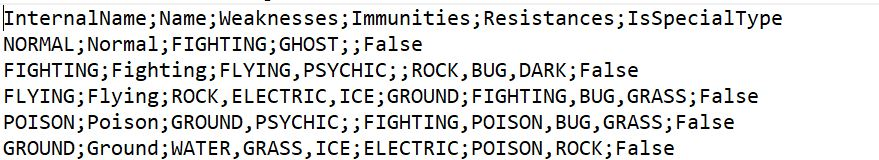
\includegraphics[scale = 0.84]{Images/fichierTexteExemple.jpg}
\caption{Exemple de fichier lu par Table}
\end{figure}

\item \textbf{VectorMethod} : Ce fichier contient des fonctions supplémentaires concernant les vecteurs. Notamment, un test vector\_in qui permet de dire si un élément est dans le vecteur, et une fonction qui permet de découper les chaînes de caractères. Cette dernière sert par exemple lors de la création des objets de type Table. 
\item \textbf{Conversion} contient une collection de fonctions permettant de convertir les objets d'un type à un autre. En effet, le compilateur MinGW fourni par notre IDE CodeBlocks ne nous laissait pas utiliser les fonction stoi, atoi stol ... qui permettent la conversion directe des types. Nous avons donc créé nos propres fonctions. Ces dernières sont généralement utilisées après la lecture des fichiers contenant des données pour convertir les std::string que la classe Table permet d'extraire (et donc de compenser le fait que Table ne soit composé que de std::string)

\item \textbf{Random} qui contient des fonctions plus simples pour faire appel à l'aléatoire. Nous avons eu des difficultés à utiliser la fonction std::uniform\_real\_distribution, c'est pourquoi nous avons créé une approximation de cette dernière à l'aide de rand()

\item  \textbf{StatSet} et \textbf{StatSetExt} sont des classes (la seconde héritant de la première) qui permettent de stocker les différentes statistiques de nos Pokemon. Lors de leur création, nous nous sommes aperçus qu'il y avait beaucoup de répétitions d'arguments liés aux points de vie, d'attaque, de défense, d'attaque spéciale, de défense spéciale et de vitesse. Nous avons aussi mis dedans la formule permettant de calculer les statistiques d'un Pokemon. \\
Si on note
\begin{itemize}
\item \textbf{Niv}, le niveau d'un Pokemon, \\
\item \textbf{PV} sa vie maximum, \\
\item \textbf{Stat} la valeur de ses autres statistiques (Attaque Défense, Attaque Spéciale, Défense Spéciale, Vitesse) (cette valeur est celle qui est valable lorsque le Pokemon est soigné), \\
\item \textbf{IV} des paramètres pour chacune des statistiques (ces derniers varient entre 0 et 31, ils sont générés aléatoirement lors de la création d'un Pokemon, ils ne sont ni visibles ni modifiables),\\
\item \textbf{EV} des paramètres pour chacune des statistiques (ces derniers varient entre 0 et 255, ils valent 0 lors de la création d'un Pokemon et varient en fonction des combats effectués, ils ne sont pas visibles par l'utilisateur, mais ce dernier peut les modifier indirectement),\\
\item \textbf{Base} des paramètres pour chacune des statistiques traduisent l'influence de l'espèce sur un Pokemon,
\end{itemize}
alors les statistiques d'un Pokemon sont définies par :
\[
Stat = \Floor{\dfrac{2 * Base + IV + \Floor{\frac{EV}{4}} * Niv + 5}{100} * Nat}
\]
\[
PV =\Floor{\dfrac{2 * Base + IV + \Floor{\frac{EV}{4}} * Niv}{100}} + Niv + 10
\]
\end{itemize}

\subsection{Structures de données (Pokemon)}
Pokemon est un répertoire qui contient l'architecture des classes que nous remplissons lorsque le programme est lancé. La plupart des classes ont un constructeur qui prend en paramètre un nom interne d'objet dont les caractéristiques sont définies dans un ou plusieurs fichiers. Le constructeur va alors utiliser la fonction Table pour lire la ligne du fichier qui l’intéresse et construire l'objet, ce qui simplifie énormément la déclaration des classes. Nous avons fait notre code de telle sorte que les arguments des uns soient les noms internes des autres ce qui permet de créer automatiquement les objets associés. 

Par ailleurs, la plupart des objets ont une structure qui n'est pas aléatoire et qui est totalement déterminée par le nom interne de l'objet, nous avons donc surchargé les operateurs == entre un objet et un std::string pour simplifier les déclarations d'égalité et rendre le code plus lisible (cela permet d'écrire par exemple if(type == ''FIRE'') ...)

Voici une description des différentes classes :

\begin{itemize}
\item \textbf{Type} contient la classe codant le Type des Pokemon ou des attaques. Les méthodes les plus importantes de cette classe sont effectiveness qui donne l'efficacité d'un Type sur un autre (par exemple, une attaque de type Eau sera très efficace contre un Pokemon de Type Feu), ainsi que getPathImage qui permet de donner l'image à afficher pour indiquer le Type d'un Pokemon.
\item \textbf{Move} contient la classe codant les attaques des Pokemon. Elle est lié au fichier ''Data/Move.txt'' qui contient une grande quantité d'arguments, parfois très complexes. Nous n'avons donc pas tout utilisé. Move contient des objets issus des classes Flag, Target et DamageCategory qui correspondent à des effets particuliers liés au attaques. Ces classes offrent une gamme de test booléen pour éviter d'avoir à gérer des notations abstraites. 
\item  \textbf{Species} contient les arguments liés à l'espèce d'un Pokemon. Nous avons décidé de sauvegarder les mouvements que peut apprendre un Pokemon (en moyenne, une centaine) sous forme de string pour ne pas utiliser inutilement de la mémoire étant donné que seul 4 sont utilisés (et sont donc converti en Move dans la classe fille Pokemon). 
\item  \textbf{Pokemon} contient principalement les fonctions qui permettent de faire varier les statistiques des Pokemon. On lui associe 2 Types, 4 Attaques, ainsi que deux structures de statistiques, l'une étant l'état normal, et l'autre l'état actuel (En effet, si un Pokemon est blessé, il n'a pas sa vie au maximum, cette information est stockée dans l'état actuel. Toutefois, si il est soigné, il revient à son état normal. Cet état normal peut aussi jouer dans le calcul des dégâts, d'où l’intérêt de le sauvegarder comme un argument). 
\end{itemize}

\begin{figure}[!h]\centering
\import{Graphiques/}{hierarchie_des_classes_de_donnees.tex}
\caption{Hiérarchie des classes de données}
\end{figure}

Les formules pour calculer les dégâts dans le vrai Pokemon sont assez compliqués :\\
Si on note :
\begin{itemize}
\item Att la statistique d'attaque si le Move est physique, l'attaque spéciale si l'attaque est spéciale
\item Def la statistique de défense si le Move est physique, l'attaque spéciale si l'attaque est spéciale
\item Power le pouvoir de base (statistique lié à Move)
\item Weather l'effet du temps
\item Badge l'effet lié aux badges de l'utilisateur
\item Critical l'effet bonus aléatoire 
\item random , un nombre entre 0.85 et 1
\item STAB, l'effet bonus si le Pokemon est du même type que son attaque
\item Type, l'effet du type de l'attaque sur le Pokemon
\end{itemize}
alors 
\[
Damage = \Floor{\left(\dfrac{\left(\dfrac{2 * Niv}{5} + 2\right) * Power * \dfrac{Att}{Def}}{50} + 2 \right) * Modifier}
\]
avec
\[
Move = Targets * Weather * Badge * Critical * random * STAB * Type * Other
\]
nous avons donc choisi de faire des simplifications car il nous était impossible de coder tout ces effets qui ont été rajoutés dans les différentes versions du jeu depuis plusieurs décennies.
\newpage

\subsection{Structure du jeu (Battle)}

\begin{figure}[!h]\centering
\import{Graphiques/}{structure_du_jeu.tex}
\caption{Hiérarchie des classes de données}
\end{figure}

Battle est un répertoire qui contient les fonctions liées aux fonctionnements des combats. Nous avons choisi de séparer les effets visuels (stockés dans Graphics) du système du jeu en lui même afin de créer des classes de combats qu'on lance via la méthode start et qui sont indépendantes. Nous avons préféré éviter d'avoir des codes trop long avec des fenêtres graphiques car le mécanisme interne des combats est complexe et cela aurait été une source d'erreur.


\subsection{Fonctions graphiques réalisées en C (Graphics)}


Graphics est un répertoire contenant toutes les fonctions graphiques gérant l'interface. Nous avons tenu à bien segmenter le code et à créer des fonctions qui se contentent d'afficher mais ne touchent pas à nos arguments. Nous avons fait seulement deux entorses à cette règle par souci de simplicité. Il s'agit de 
 hpallydecrease et hpfoedecrease qui impactent respectivement la barre de vie du Pokemon allié et celle du Pokemon ennemi en combat.
 
Nous avons distingué deux principales natures de graphiques:

\begin{itemize}
\item Field, qui permet de générer la carte du jeu sur laquelle se déplace le personnage. Nous avons codé le déplacement du personnage et la rencontre de Pokemon sauvages. A l'aide de la touche Espace, le joueur peut afficher un menu lui permettant notamment de consulter ses Pokemon.
\item l'interface de combat, comprenant l'écran de combat et les menus associés. L'interface de combat est créée à l'aide de macro \#define permettant de redefinir sur chacune de nos fonctions graphiques les mêmes éléments à quelques variations près. Pour créer une interface de combat, il faut afficher l'arrière plan, la base du Pokemon ennemi, celle du Pokemon allié, le Pokemon ennemi, le Pokemon allié, la barre de menus présente en bas, les deux boites de data contenant la vie des Pokemon, ainsi que leurs nom, leurs niveau (Level), l'image de leurs barre de vie, et enfin la vie sous forme d'un entier pour le Pokemon allié.
\end{itemize}

Les menus proposés permettent entre autres de choisir le Pokemon qui combat, de s'enfuir, ou de choisir ses attaques dans le cas du choix du fight menu. Grâce à un usage de la technique de double buffering, alors même que les menus sont gérés par des fonctions différentes, la transition à l'écran s'effectue sans changement visuel pour l'utilisateur.

La plupart des fonctions utilisées sont des fonctions soit de type void, soit renvoyant un flag. Par exemple, l'affichage d'un menu peut être un flag demandé par un utilisateur, tel le Fight menu lors d'un clic sur Fight. Toutes ces fonctions prennent en paramètre l'écran, et décident tour à tour ce qu'elles appliquent dessus. A l'opposé de ces flags volontaires, certains flags telle la rencontre avec un Pokemon, simulée par une loi binomiale, sont involontaires.
Une des grosses difficultés du code était de ne pas avoir une seule fonction massive de plusieurs milliers de lignes. Nous avons donc compartimenté notre code en de nombreuses fonctions, ce qui a également aidé au respect du principe de segmentation du code évoqué plus haut. On peut par exemple l'observer dans la fonction LaunchFoePokemon, où 5 lignes de SET\_BATTLE servent à faire appel à de nombreuses fonctions définies dans Battle.

\newpage
\pagestyle{empty}

\import{Parties/}{Conclusion}

\end{document}

%\begin{lstlisting}
%int main()
%{
%	int a = 3;
%	std::string mot = ''je suis'';
%	return 0;
%}
%\end{lstlisting}